\documentclass[11pt]{article}
\usepackage[margin=1in]{geometry}
\usepackage{graphicx}
\usepackage{microtype}
\usepackage{verbatim}
\usepackage{amsmath}
\usepackage{nicefrac}
\usepackage[colorlinks=false, hidelinks]{hyperref}
\usepackage{caption}
\usepackage{subcaption}
\usepackage{listings}
\usepackage{harmony}
\usepackage{wasysym}

\begin{document}

\title{LFSR and ASG Pseudorandom Number Generators\\Embedded System Design, Lab 5}
\date{October 22, 2015}
\author{Ben Lorenzetti}
\maketitle

\tableofcontents

\clearpage

\section{Objectives and Problem Descriptions}
\subsection{8-Bit Linear Feedback Shift Register (LFSR)}
\label{problem-1-specs}

\subsection{Alternating Step Generator (ASG)}
\label{problem-2-spces}

\section{Procedure}
\subsection{Reading Assignments}

\subsection{LFSRs and ASGs Theory}

\begin{figure}
	\centering
	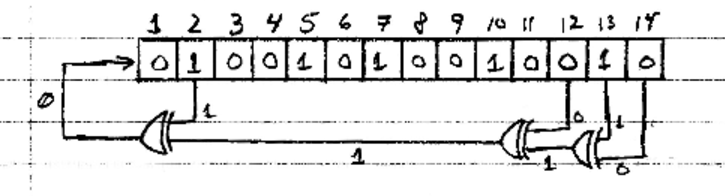
\includegraphics[width=0.7\textwidth]{Figures/14-bit-fibonacci-with-feedback-polynomial.pdf}
	\caption{A 14-bit Fibonacci LFSR with feedback polynomial $F(x)=x^{14}+x^{13}+x^{12}+x^{2}+1$}
	\label{14-bit-fibonacci-with-feedback-polynomial}
\end{figure}

\subsection{Implementation Design}

\begin{figure}
	\centering
	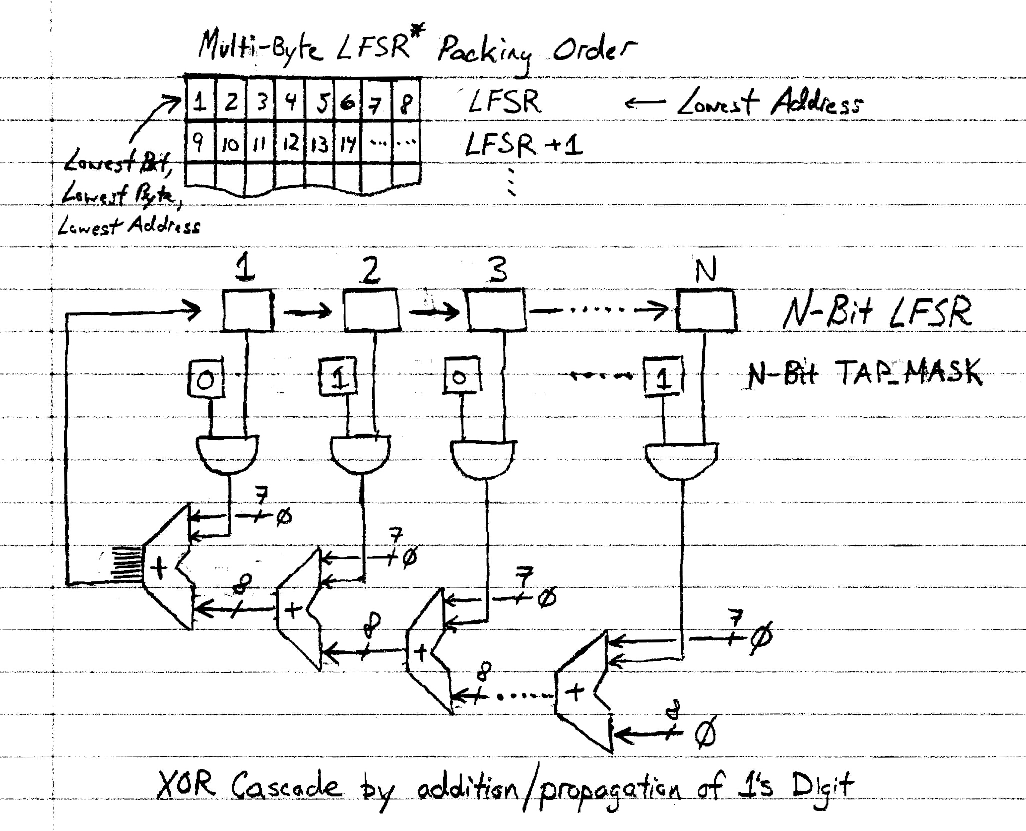
\includegraphics[width=0.9\textwidth]{Figures/fibonacci-equivalent-circuit.pdf}
	\caption{Equivalent Circuit Implementation of an Arbitrary Length Fibonacci LFSR}
	\label{fibonacci-equivalent-circuit}
\end{figure}

\begin{figure}
	\centering
	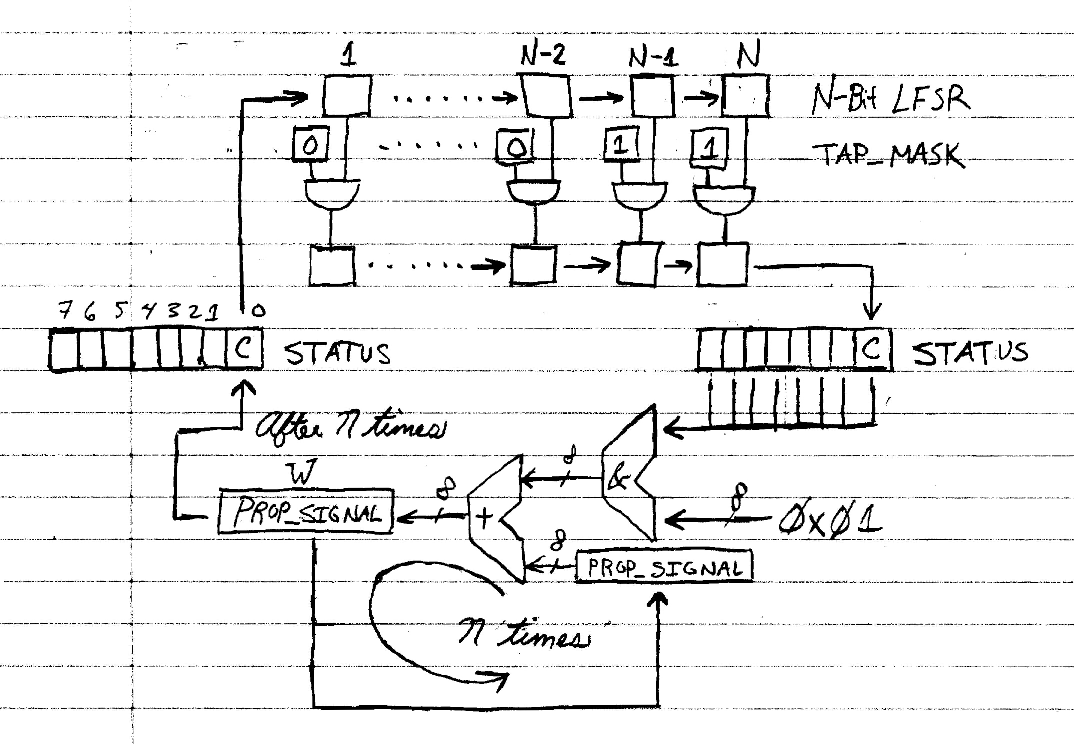
\includegraphics[width=0.9\textwidth]{Figures/xor-propagation-flowchart.pdf}
	\caption{Implementation of XOR Propagation}
	\label{xor-propagation-flowchart}
\end{figure}

\begin{figure}
	\centering
	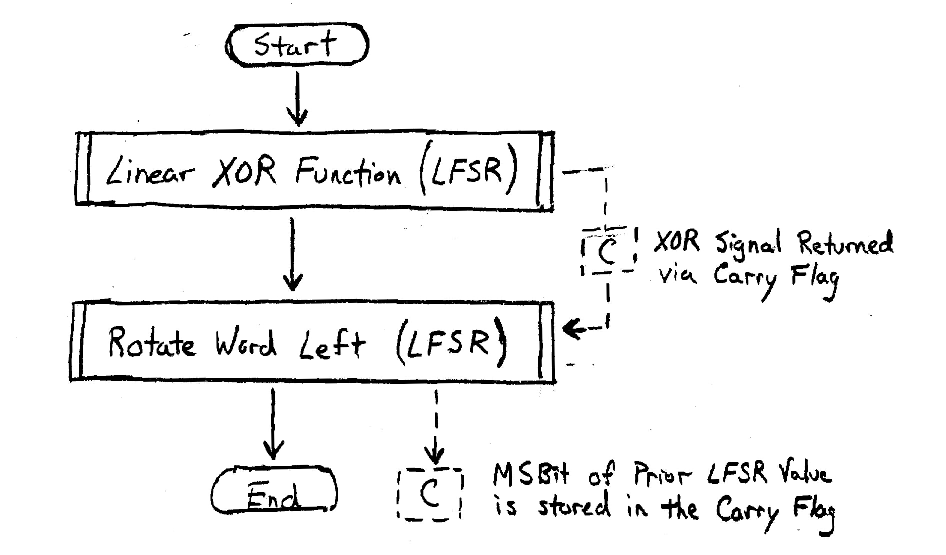
\includegraphics[width=0.6\textwidth]{Figures/cycle-lfsr-flowchart.pdf}
	\caption{Cycle LFSR Function Implementation Flowchart}
	\label{cycle-lfsr-flowchart}
\end{figure}


\subsection{Hello World Program (Delay Function)}

\subsection{Assembly Macros (Rotate Word Function)}

\subsection{XOR Propagation Function}

\subsection{8-Bit LFSR Design}

\begin{figure}
	\centering
	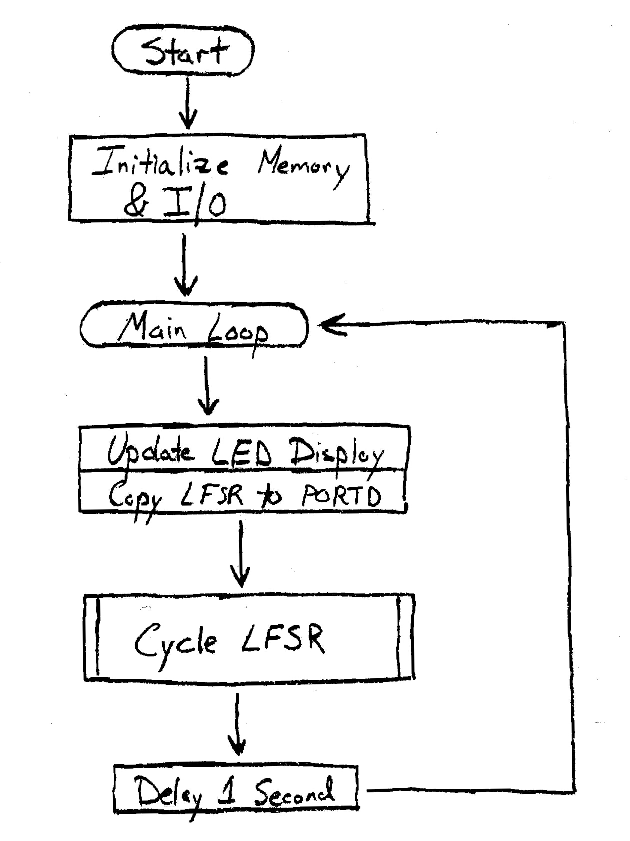
\includegraphics[width=0.35\textwidth]{Figures/8-bit-lfsr-flowchart.pdf}
	\caption{8-Bit LFSR Implementation Flowchart}
	\label{8-bit-lfsr-flowchart}
\end{figure}

\subsection{ASG Design}

\begin{figure}
	\centering
	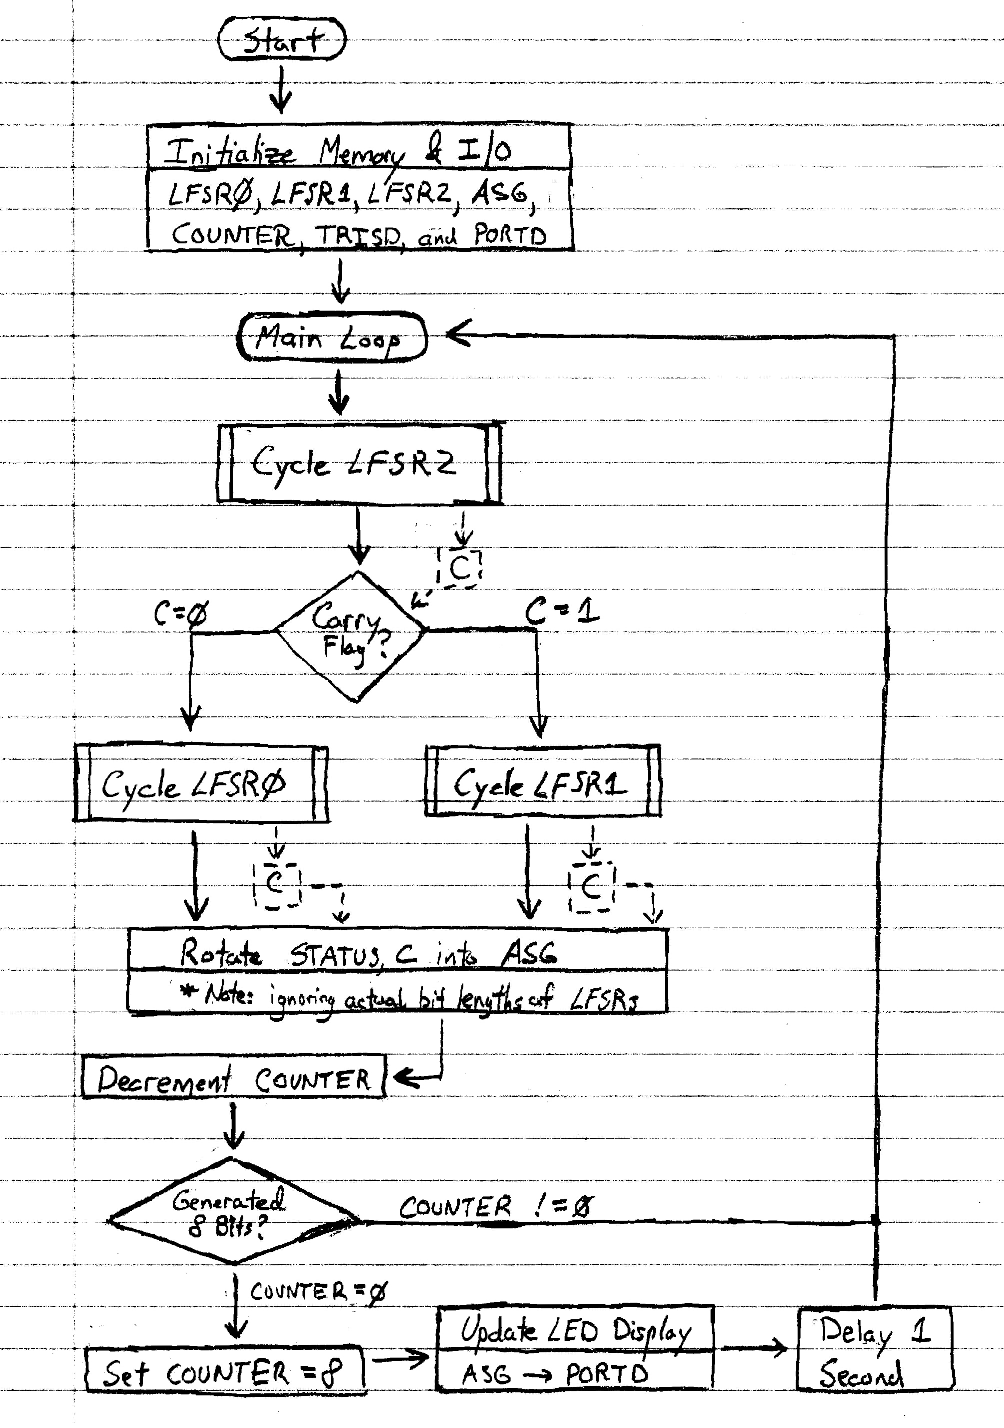
\includegraphics[width=0.6\textwidth]{Figures/alternating-step-generator-flowchart.pdf}
	\caption{Alternating Step Generator Implementation}
	\label{alternating-step-generator-flowchart}
\end{figure}

\section{Expected Results}

\subsection{3-Bit LFSR Demonstration}

\subsection{8-Bit LFSR Demonstration}

\subsection{ASG Demonstration}

\section{Experiment and Design Revisions}

\subsection{Addition of Macros}

\subsection{Use of Carry Flag between Functional Blocks}

\section{Observations}

\subsection{Observations}

\section{Discussion}

\subsection{Discussion of Results}

\subsection{Carry Flag and PIC Design}

\section{Exercises}

\clearpage
\section{Implementation Code}

\subsection{8-Bit LFSR}
\label{lsfr-code}

\lstinputlisting[breaklines]{Eight-Bit-LFSR/lfsr.asm}


\clearpage
\subsection{Alternating Step Generator}
\label{asg-code}

\lstinputlisting[breaklines]{Alternating-Step-Generator/asg.asm}



\end{document}
